\documentclass[12pt,a4paper]{article}
\usepackage{rmpackages}																% usual packages
\usepackage{rmtemplate}																% graphic charter
\usepackage{rmexocptce}																% for DS with cptce eval

%\cfoot{} 													% if no page number is needed
\renewcommand\arraystretch{1.7}		% stretch table line height

\begin{document}

\begin{header}
Chapitre 3 -- Du macroscopique au microscopique
\end{header}

Les deux premiers chapitres nous ont permis de décrire et caractériser la matière à notre échelle, l'échelle \textbf{macroscopique}.
L'objectif de ce chapitre est de modéliser la matière à l'échelle des particules qui la compose, l'échelle \textbf{microscopique}.

\section{Vers le microscopique}

\subsection{Identifier les images}

Les images ci-dessous représentent (dans le désordre) : un chat, un virus, un cheveu, des atomes, un flocon de neige, des cellules animales, une abeille et un morceau de molécule d'ADN.

\emph{Écris sous chaque image ce qu'elle représente.}

\begin{figure}[h]
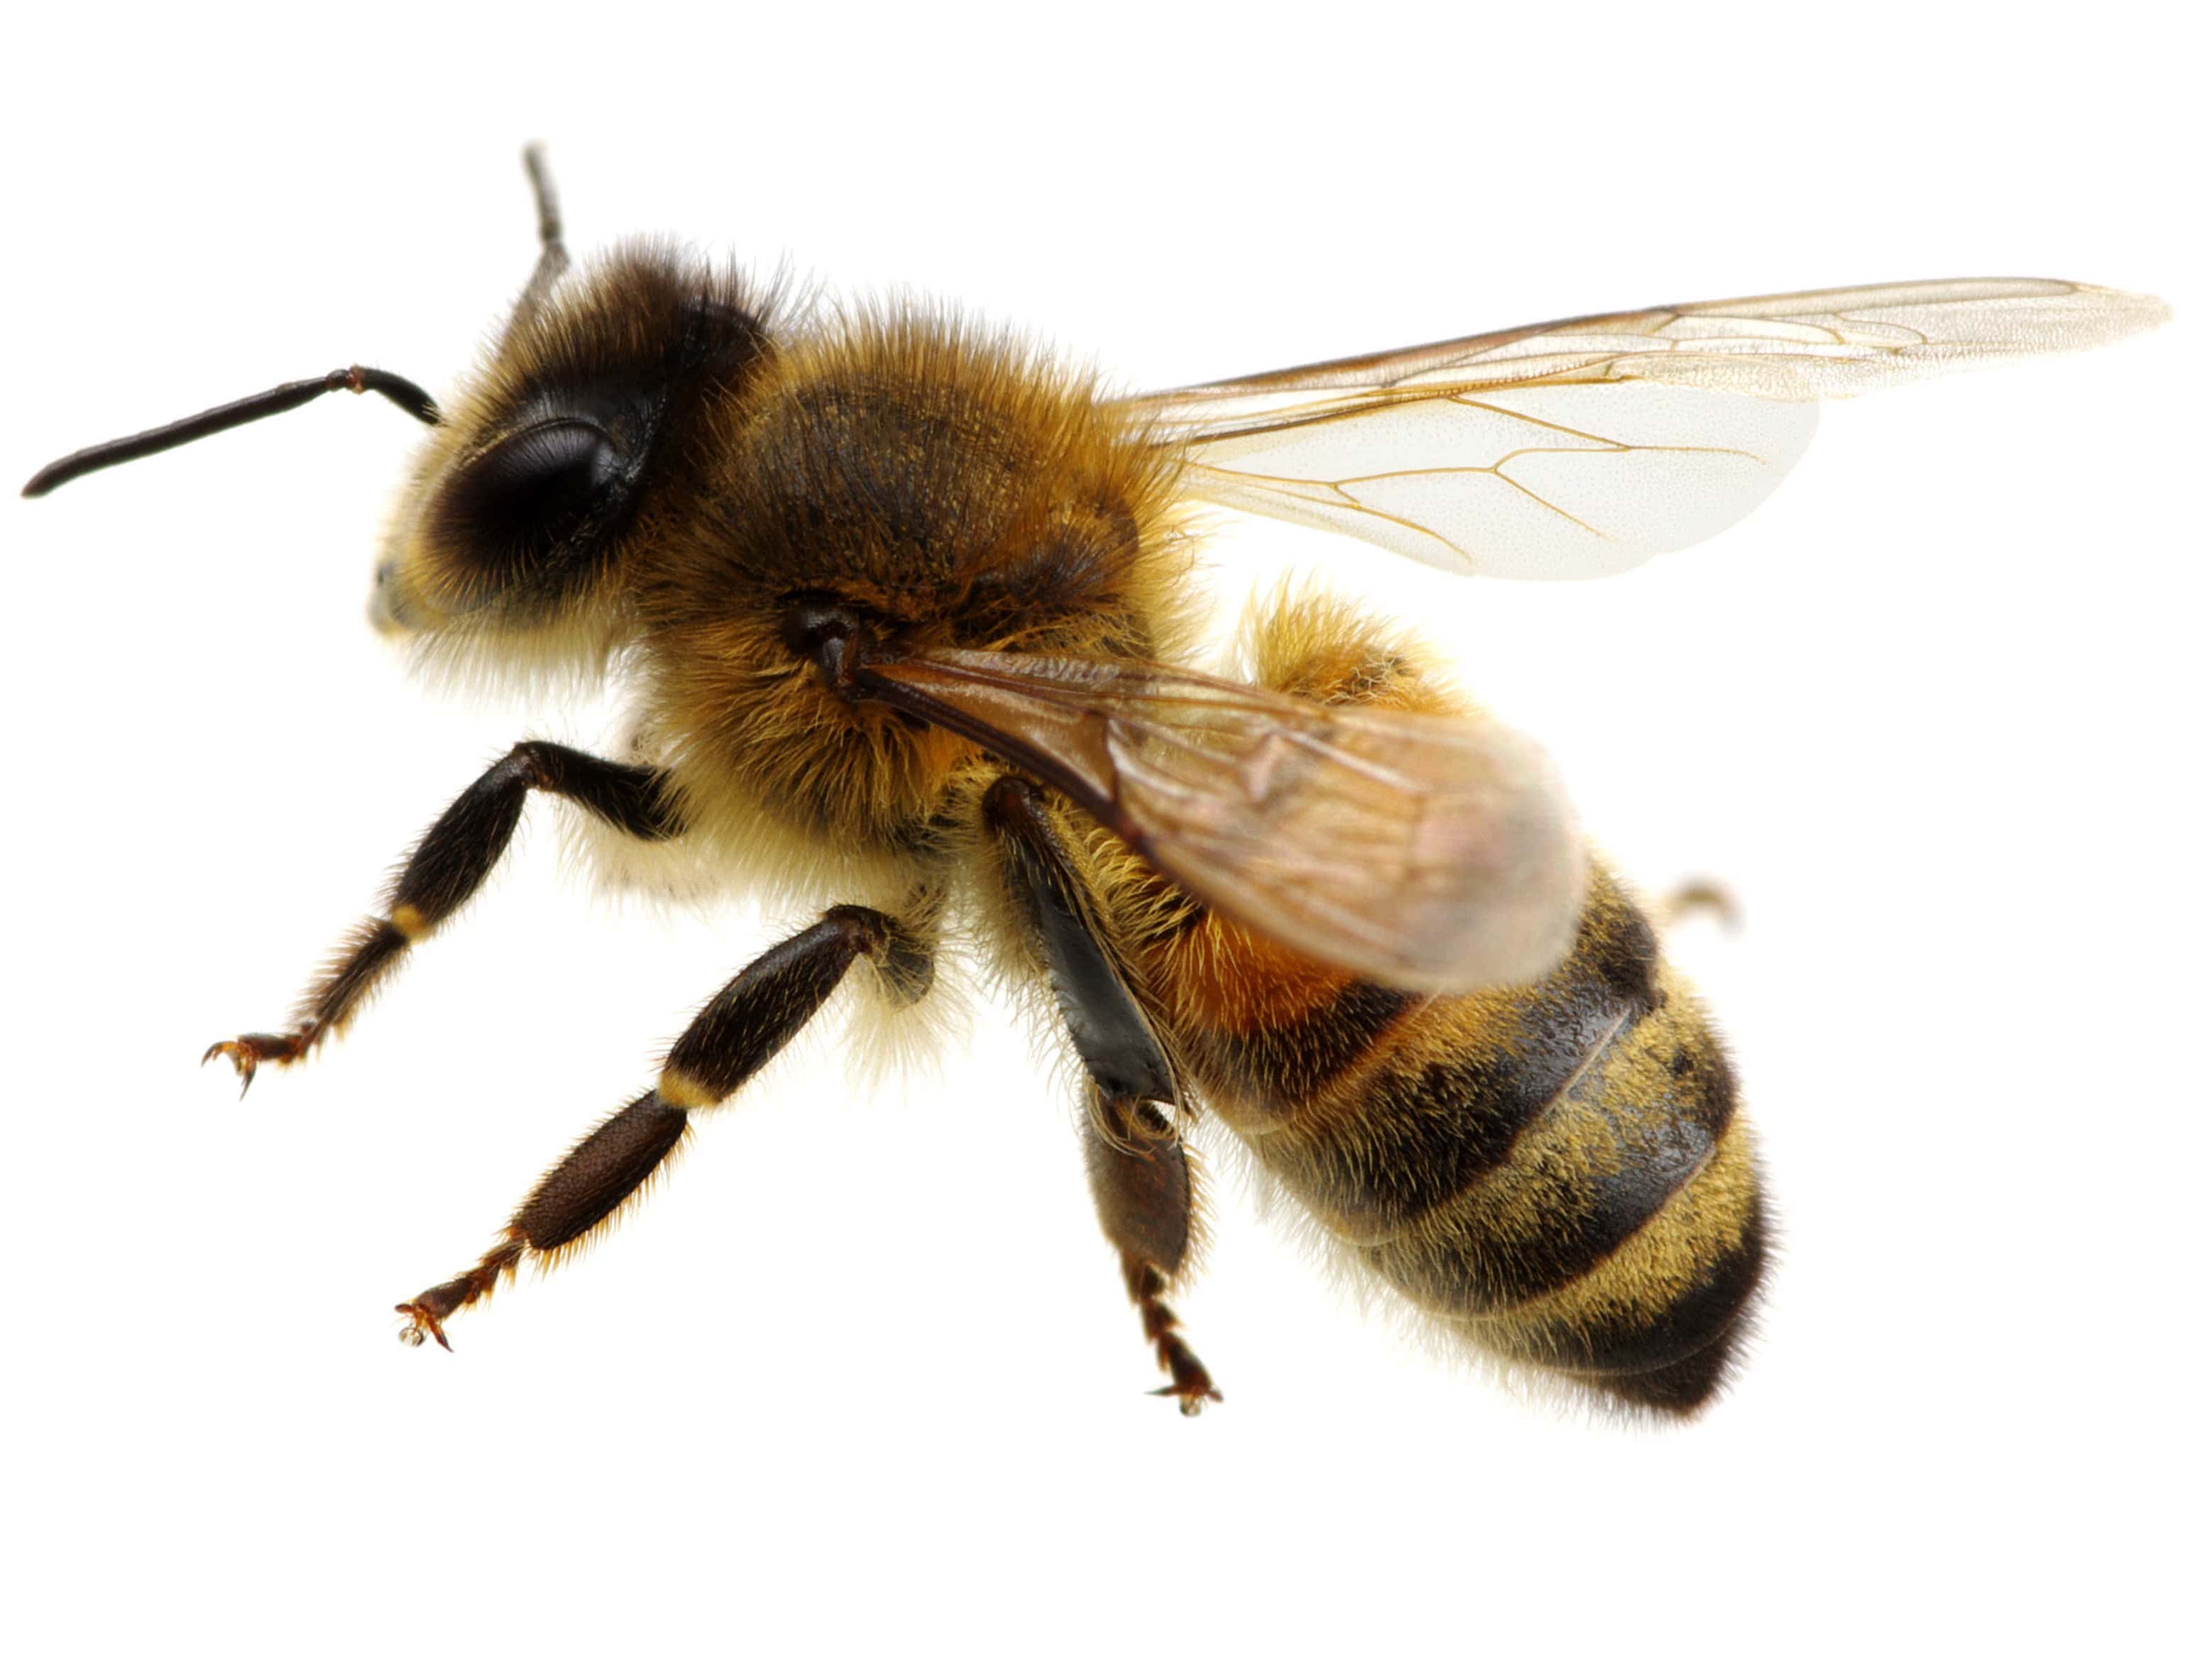
\includegraphics[height=100pt]{images/abeille.jpg}
\hfill
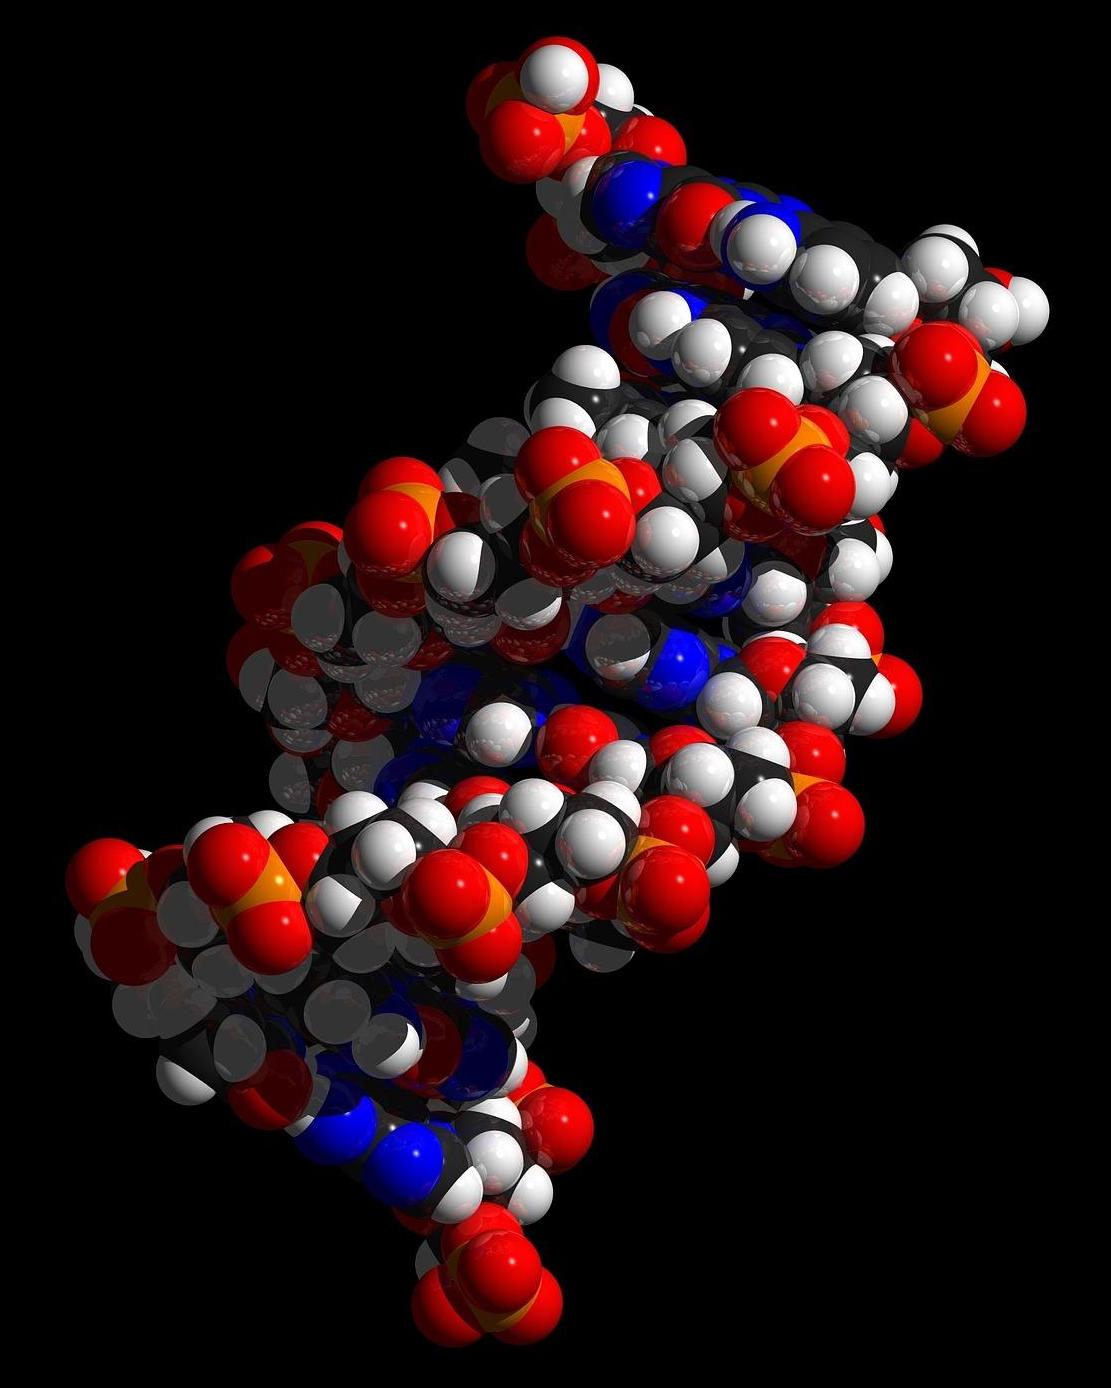
\includegraphics[height=100pt]{images/adn.jpg}
\hfill
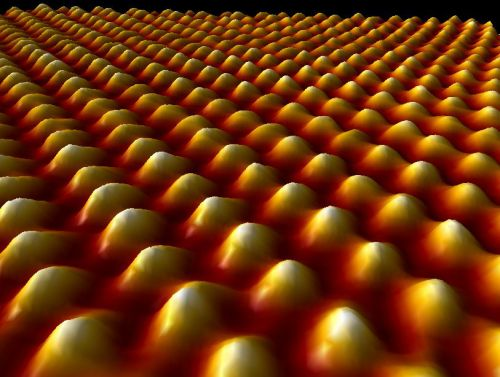
\includegraphics[height=100pt]{images/atoms.jpg}
\hfill
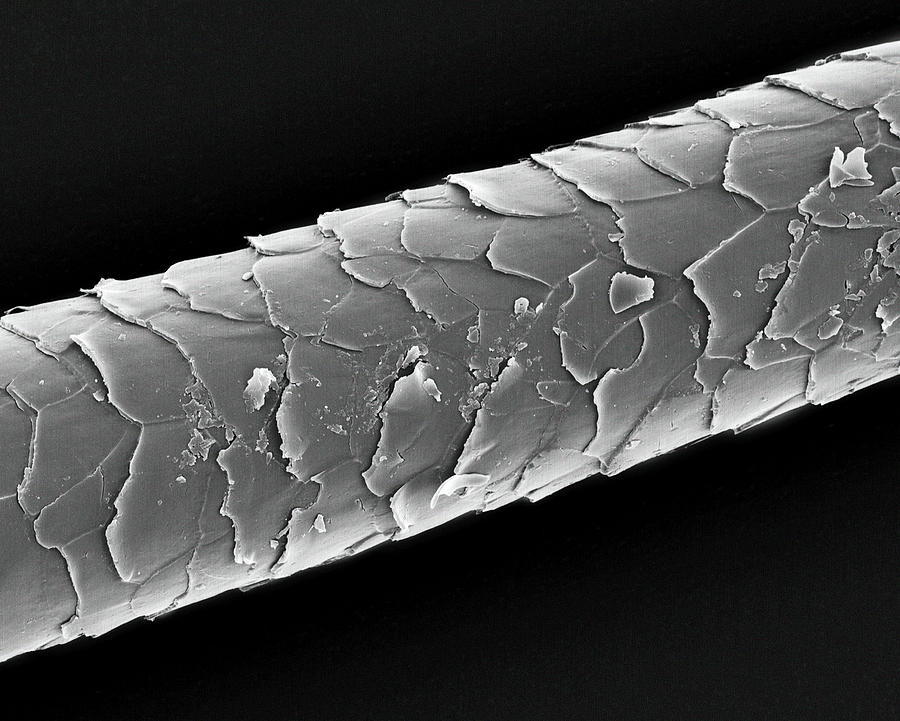
\includegraphics[height=100pt]{images/hair.jpg}

\vspace{50pt}

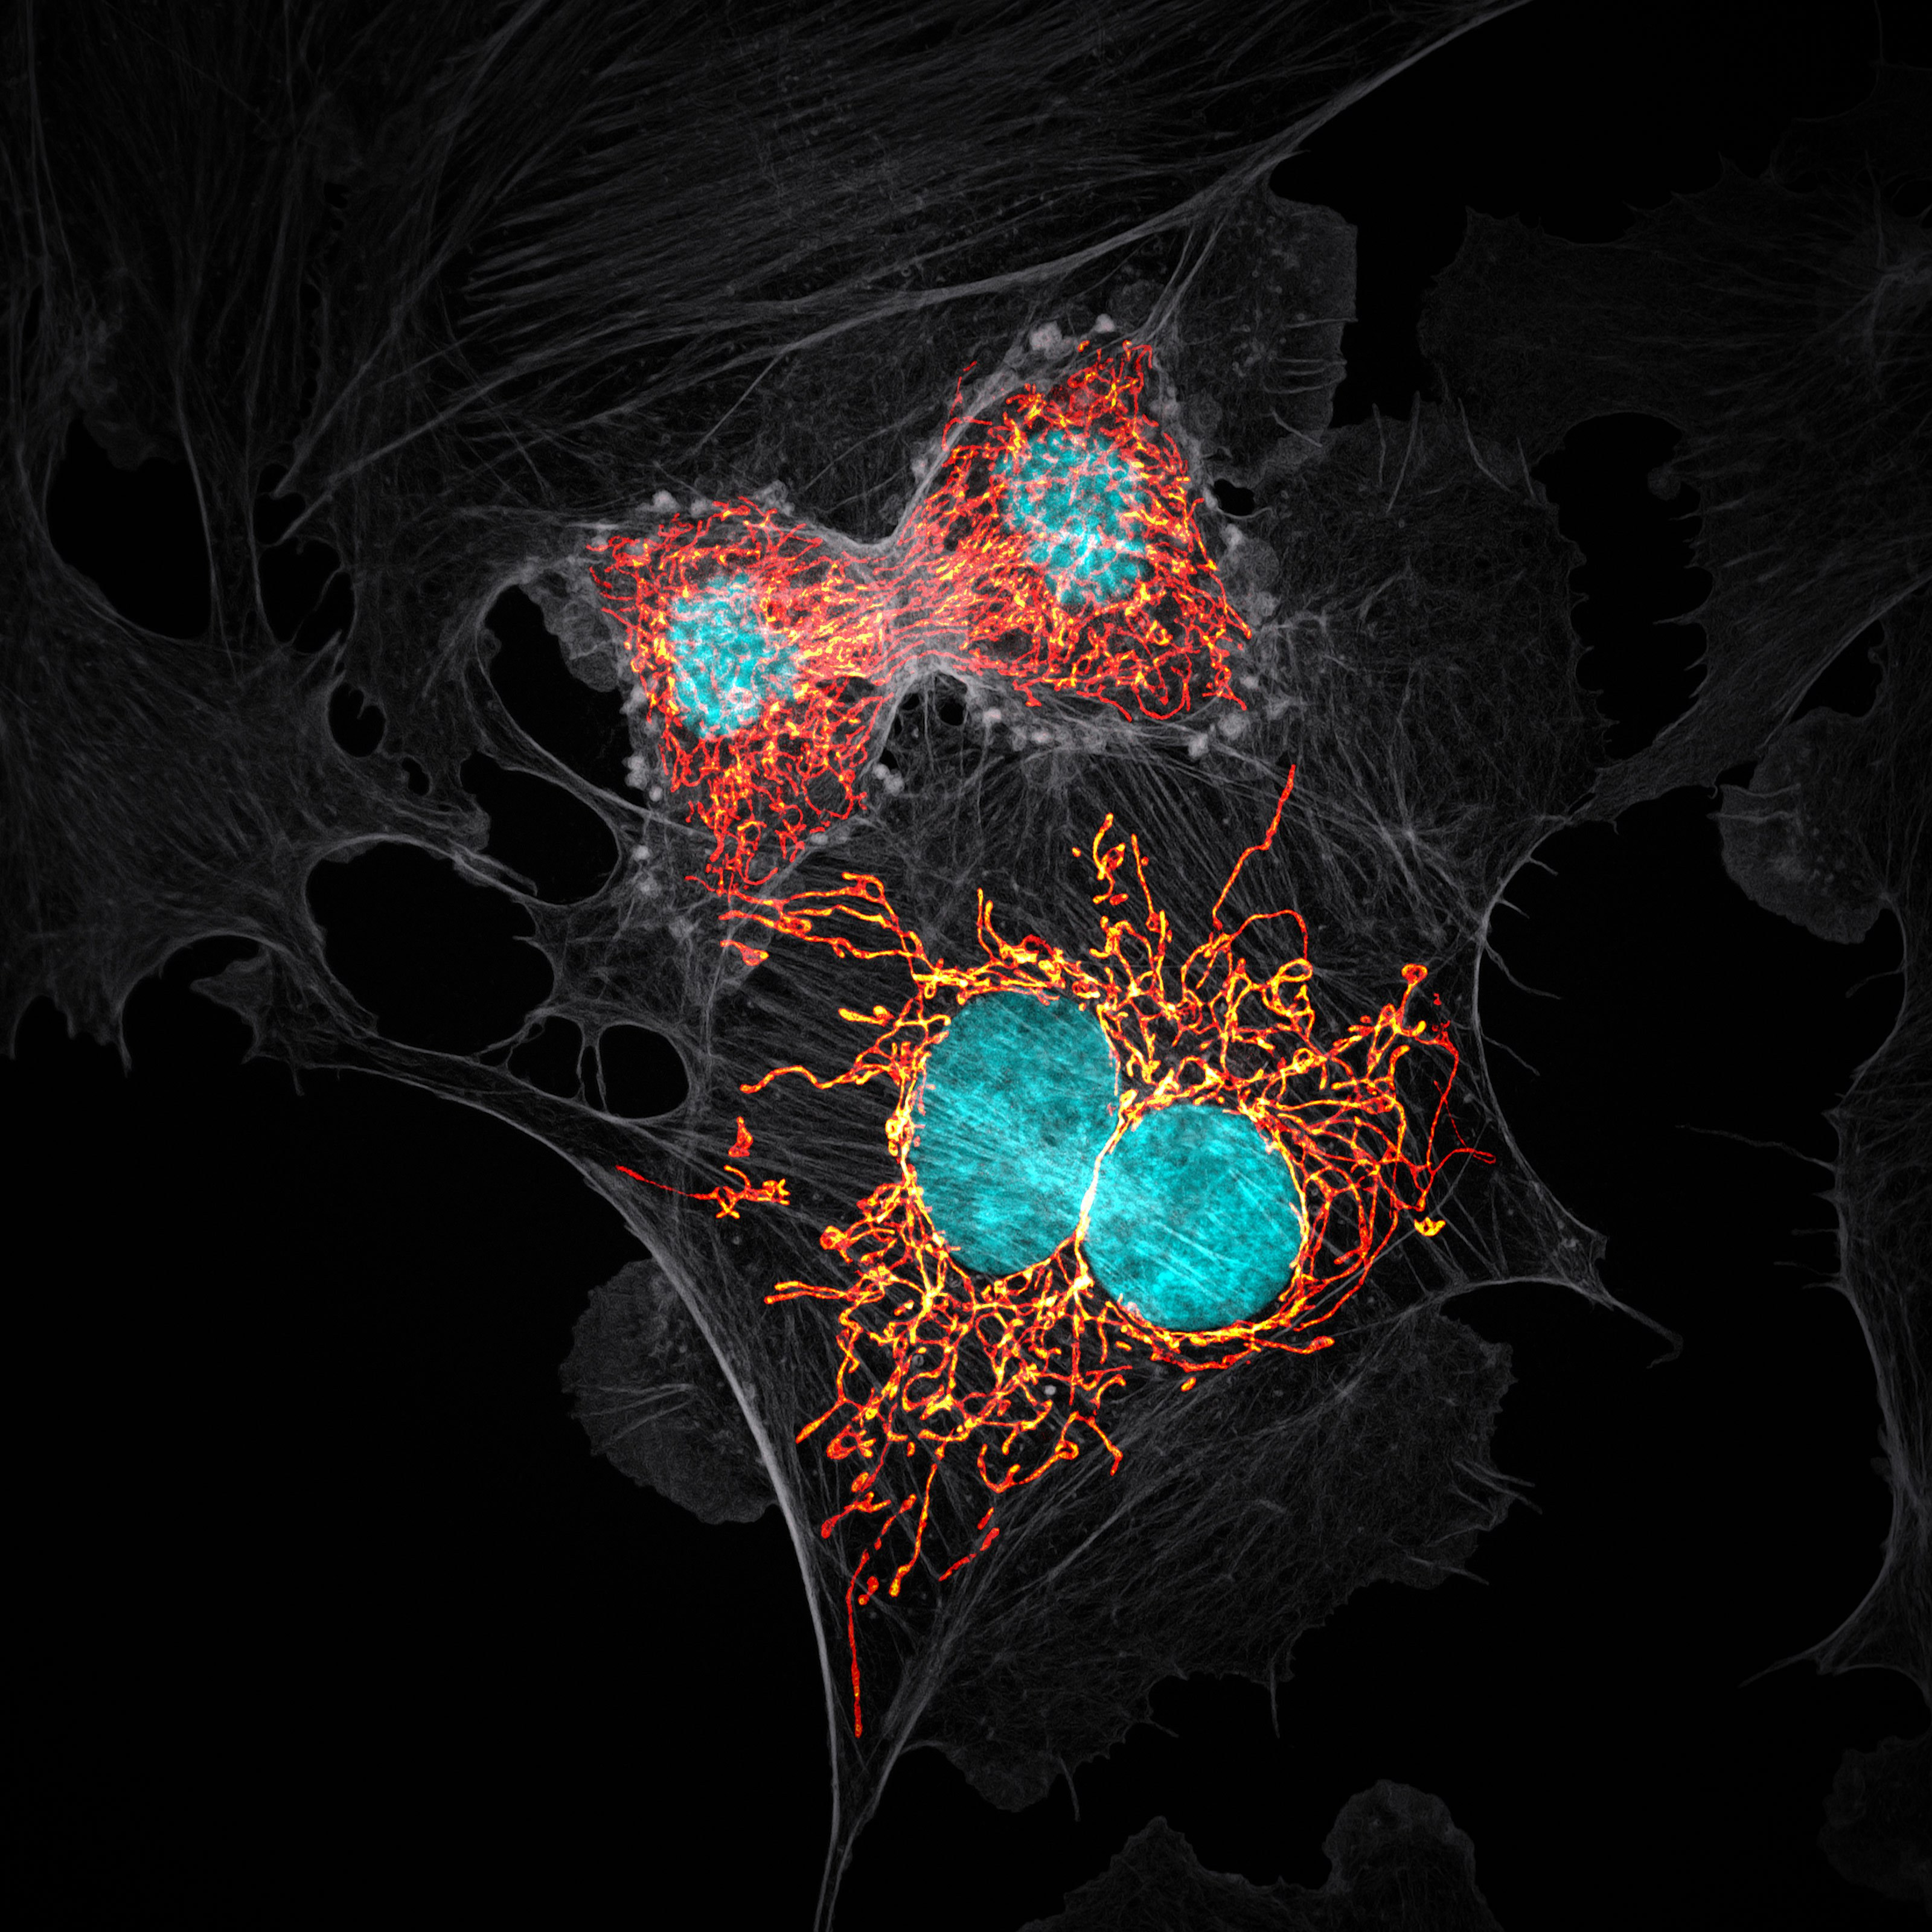
\includegraphics[height=100pt]{images/bpae_cell_mitosis.jpg}
\hfill
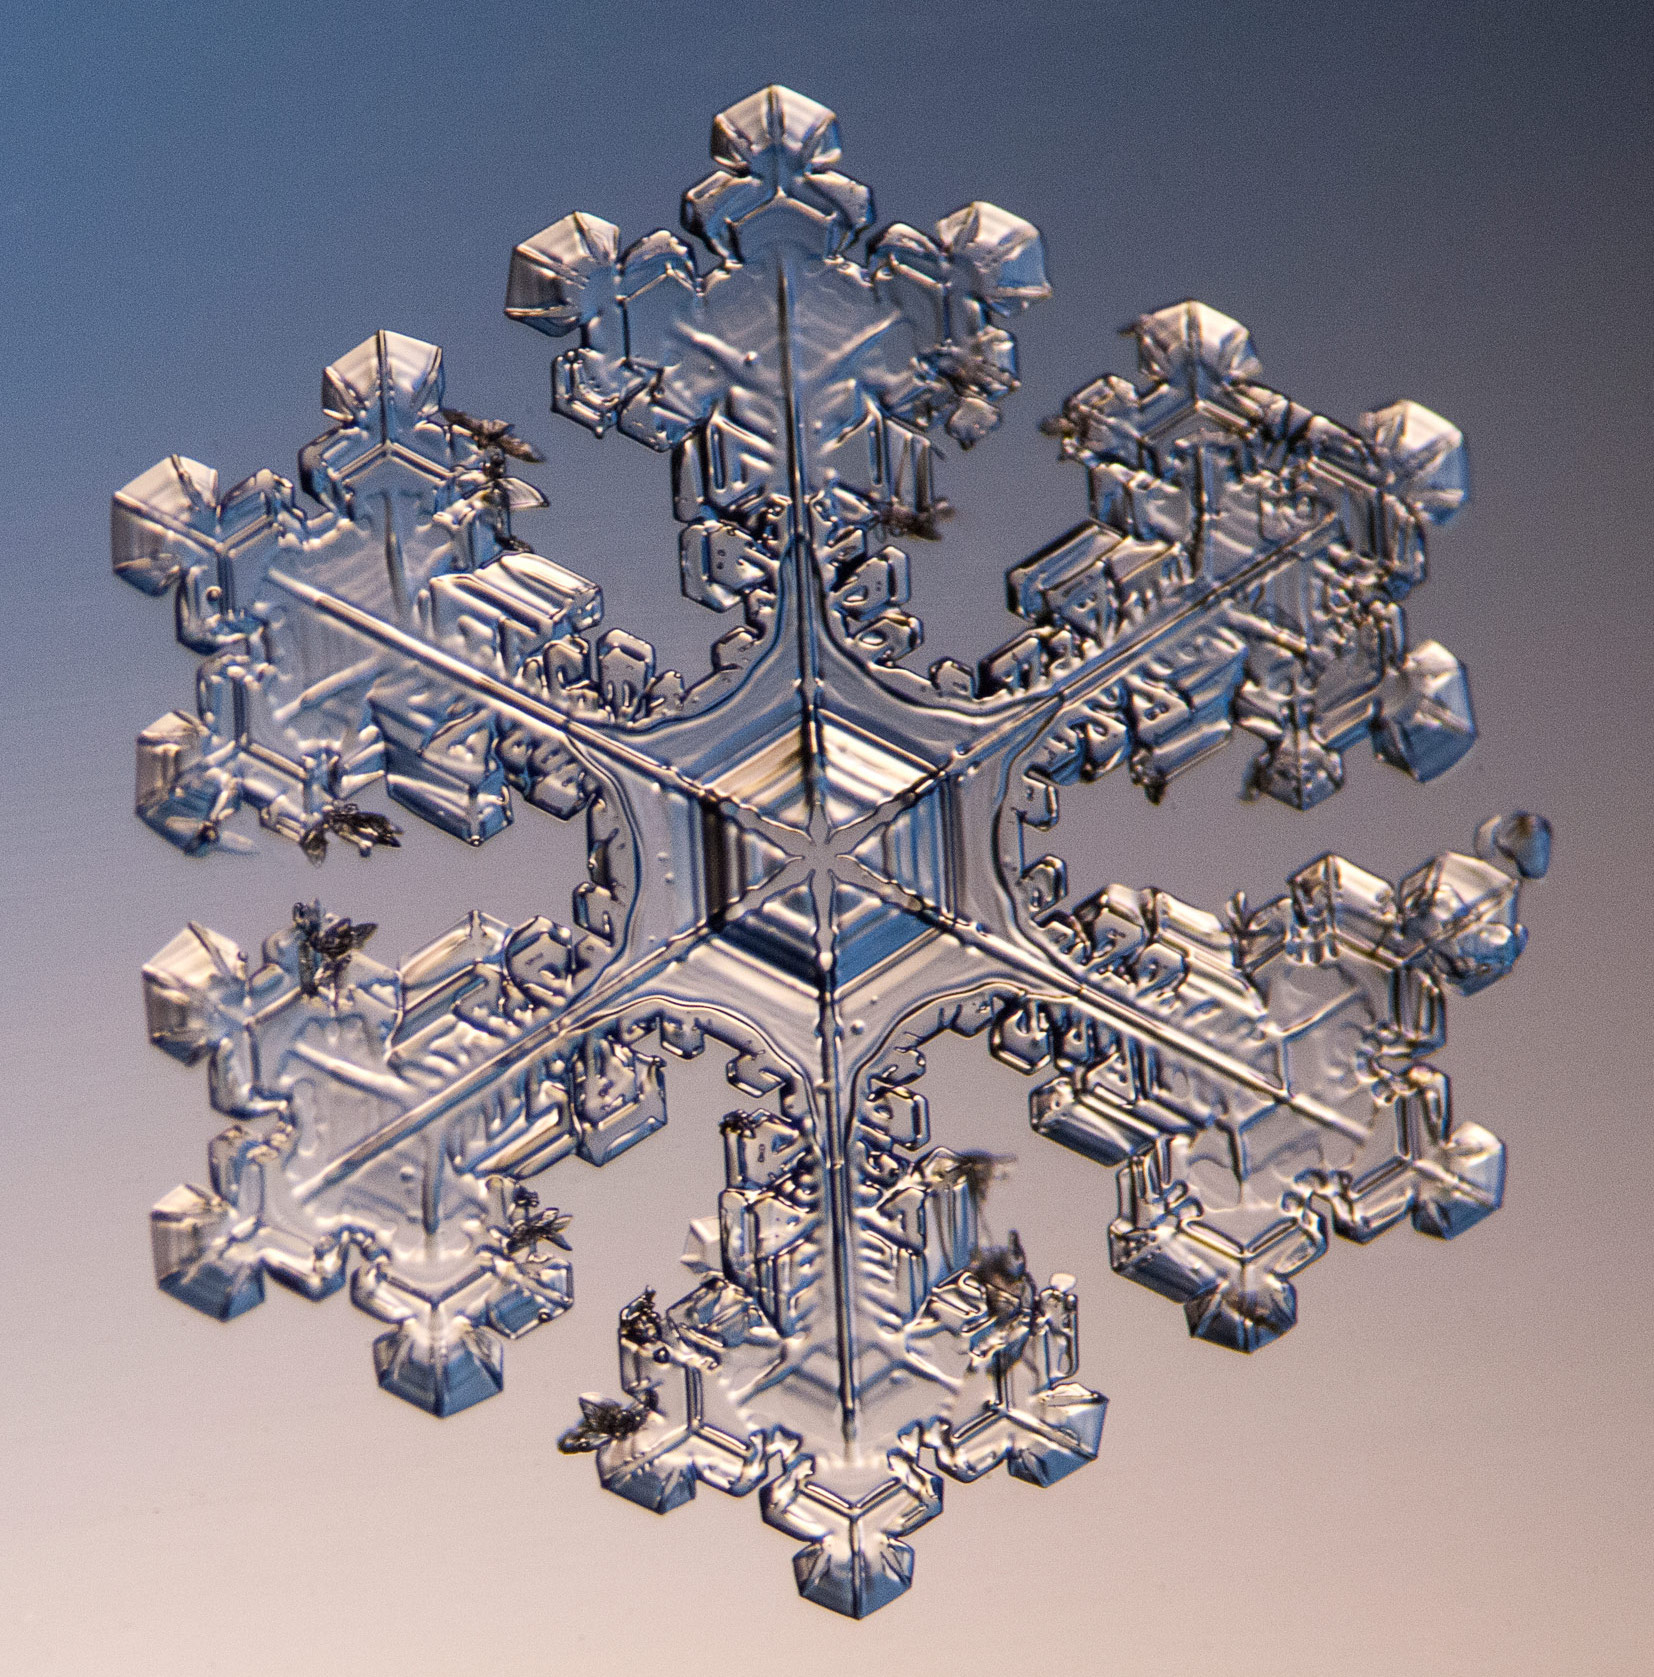
\includegraphics[height=100pt]{images/flocon_neige.jpg}
\hfill
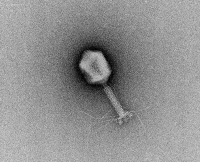
\includegraphics[height=100pt]{images/virus.jpg}
\hfill
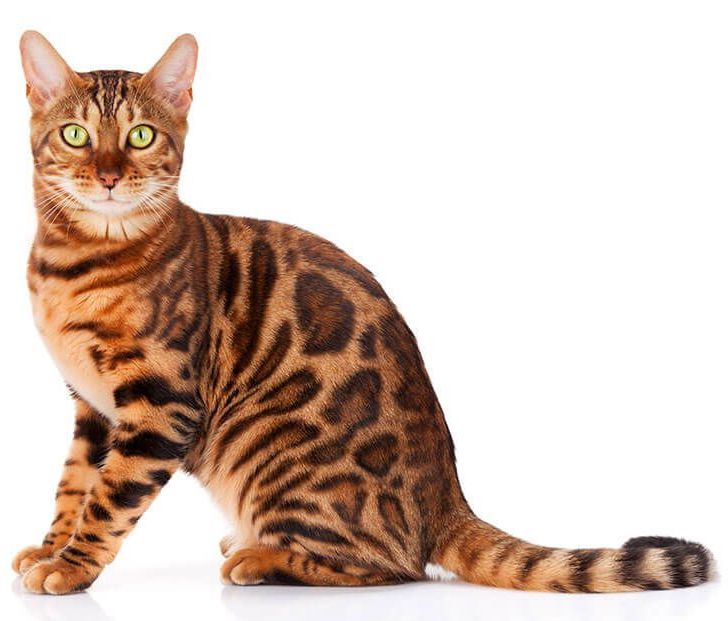
\includegraphics[height=100pt]{images/chat_bengal.jpg}
\end{figure}

\vspace{20pt}


\subsection{Du plus grand au plus petit}

\emph{Réécris la liste des éléments précédents en les classant par taille du plus grand au plus petit.}

\newpage

\subsection{Quelle est leur taille ?}

\emph{Complète le tableau.}

\begin{table}[h]
\center
\begin{tabular}{>{\centering}p{0.2\textwidth} | p{0.4\textwidth}<{\centering}}
\textbf{Taille}  & \textbf{Élément} \\
\hline\hline
\unit{75}{\micro\meter} & \\ \hline
\unit{5}{\deci\meter} & \\ \hline
\unit{2}{\milli\meter} & \\ \hline
\unit{2}{\nano\meter} & \\ \hline
\unit{0{,}1}{\nano\meter} & \\ \hline
\unit{10}{\micro\meter} & \\ \hline
\unit{100}{\nano\meter} & \\ \hline
\unit{1}{\centi\meter} &
\end{tabular}
\end{table}

\subsection{Et en mètre, ça fait combien ?}

\emph{Complète le tableau.}

\begin{definition}
\begin{itemize}
\item[•] $\unit{1}{\micro\meter} = \unit{1\times10^{-6}}{\meter}$
\item[•] $\unit{1}{\nano\meter} = \unit{1\times10^{-9}}{\meter}$
\end{itemize}
\end{definition}

\begin{table}[h]
\center
\begin{tabular}{>{\centering}p{0.2\textwidth} | p{0.4\textwidth}<{\centering}}
\textbf{Taille} & \textbf{Valeur en mètre} \\
\hline\hline
\unit{75}{\micro\meter} & \\ \hline
\unit{5}{\deci\meter} & \\ \hline
\unit{2}{\milli\meter} & \\ \hline
\unit{2}{\nano\meter} & \\ \hline
\unit{0{,}1}{\nano\meter} & \\ \hline
\unit{10}{\micro\meter} & \\ \hline
\unit{100}{\nano\meter} & \\ \hline
\unit{1}{\centi\meter} &
\end{tabular}
\end{table}

\begin{conseil}
Un rappel sur les puissances de 10 sera fait en classe.
\end{conseil}

\subsection{Du macroscopique au microscopique}

\emph{Résume les résultats précédents en plaçant les différents éléments autour de l'échelle de taille et en réécrivant pour chacun son nom et sa taille.}

\begin{figure}[h!]
\center
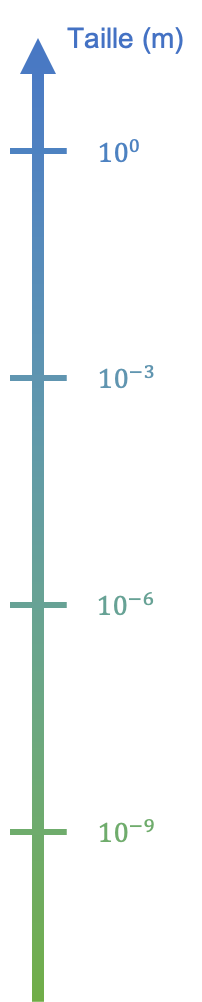
\includegraphics[scale=1.25]{images/chap3_scales.png}
\end{figure}

\section{Modèle microscopique de la matière}

\begin{definition}
Une espèce chimique est constituée d'un très grand nombre d'entités chimiques, c'est à dire d'un très grand nombre d'atomes, d'ions, ou de molécules.
\end{definition}

\emph{Pour chaque espèce chimique ci-dessous, dire si elle est constituée d'atomes, de molécules, de cations ou d'anions.}
\begin{table}[h]
\center
\begin{tabular}{l c p{0.18\textwidth} l c p{0.18\textwidth} l c p{0.18\textwidth}}
C  & : & & $\eau$ & : & & $\chlorure$ & : & \\
$\saccharose$  & : & & $\ionsodium$ & : & & Fe & : & \\
$\ioncuivreII$  & : & & $\sulfate$ & : & & $\diazote$ & : & \\
\end{tabular}
\end{table}

\emph{Complète les définitions ci-dessous.}

\begin{definition}
\begin{itemize}
\begin{spacing}{1.5}
\item[•] Un \textbf{atome} est une entité chimique électriquement \underline{\color{red_c} neutre neutre} constituée d'un noyau chargé \underline{\color{red_c} positivement positivement} et d'\underline{\color{red_c} électrons électrons} chargés négativement.
\item[•] Une \textbf{molécule} est une entité chimique électriquement \underline{\color{red_c} neutre neutre} formée de plusieurs \underline{\color{red_c} atomes atomes} liés entre eux.
\item[•] Un \textbf{ion} est une entité chimique électriquement \underline{\color{red_c} chargée chargée}.
\item[•] Un \textbf{cation} est un \underline{\color{red_c} ion ion } chargé \underline{\color{red_c} positivement positivement}.
\end{spacing}
\item[•] Un \textbf{anion} est un \underline{\color{red_c} ion ion } chargé \underline{\color{red_c} négativement négativement}.
\end{itemize}
\end{definition}

Quand on écrit la formule chimique d'une espèce ionique, on indique le nombre de charges portées par les ions qui la compose : chaque ion de cuivre II $\ioncuivreII$ porte deux charges positives.

\section{Électroneutralité de la matière à l'échelle macroscopique}

\subsection{Les solides ioniques}

\begin{exemple}
Le sel de table a pour formule chimique NaCl : c'est le chlorure de sodium.
C'est un solide ionique composé :
\begin{itemize}
\item[•] de cations sodium $\ionsodium$ possédant une charge positive ;
\item[•] d'anions chlorure $\chlorure$ possédant une charge négative.
\end{itemize}
Le chlorure de sodium a donc autant de charges positives que de charges négatives (une de chaque), il est neutre.
\end{exemple}

\begin{exemple}
Le nigari, ou chlorure de magnésium est un solide ionique composé :
\begin{itemize}
\item[•] de cations magnésium $\ionmagnesiumII$ possédant deux charges positives ;
\item[•] d'anions chlorure $\chlorure$ possédant une charge négative.
\end{itemize}
Pour qu'il soit neutre, il faut deux fois plus d'anions chlorure $\chlorure$ que de cation magnésium $\ionmagnesiumII$ : en effet, le nombre de charges positives doit être égal au nombre de charges négatives.
La formule chimique du chlorure de magnésium est donc $\chloruredemagnesium$.
\end{exemple}

\begin{definition}
Un solide ionique est toujours électriquement \underline{\color{red_c} neutre neutre}.
\end{definition}

Par convention on écrit la formule chimique d'un solide ionique en commençant par le cation.

\subsection{Applications}

\begin{multicols}{2}
{
\center
\renewcommand*{\arraystretch}{1}
\begin{tabular}{l | c}
\textbf{Nom} & \textbf{Formule chimique} \\
\hline\hline
ion hydrogène 	& $\ionhydrogene$ \\
ion sodium     	& $\ionsodium$ \\
ion magnésium	& $\ionmagnesiumII$ \\
ion chlorure		& $\chlorure$ \\
ion potassium 	& $\ionpotassium$ \\
ion fer II			 	& $\ionferII$ \\
ion fer III			 	& $\ionferIII$ \\
ion cuivre II	 	& $\ioncuivreII$ \\
ion iodure		 	& $\iodure$ \\
ion hydroxyde	& $\hydroxyde$ \\
ion sulfate			& $\sulfate$ \\
ion permanganate & $\permanganate$
\end{tabular}
}

\emph{À l'aide des deux exemples précédents et du tableau ci-contre, écris la formule chimique des solides ionique suivants :}

\noindent
\begin{tabular}{l l}
\textbullet{} iodure de potassium 				& : \\
\textbullet{} chlorure d'hydrogène 				& : \\
\textbullet{} permanganate de potassium	& : \\
\textbullet{} sulfate de cuivre II					& : \\
\textbullet{} chlorure de fer III						& : \\
\textbullet{} sulfate de fer III						& :
\end{tabular}
\end{multicols}

\end{document}